\section{Interface}
\label{sect:kegg_interface}

\begin{figure}
    \center{
        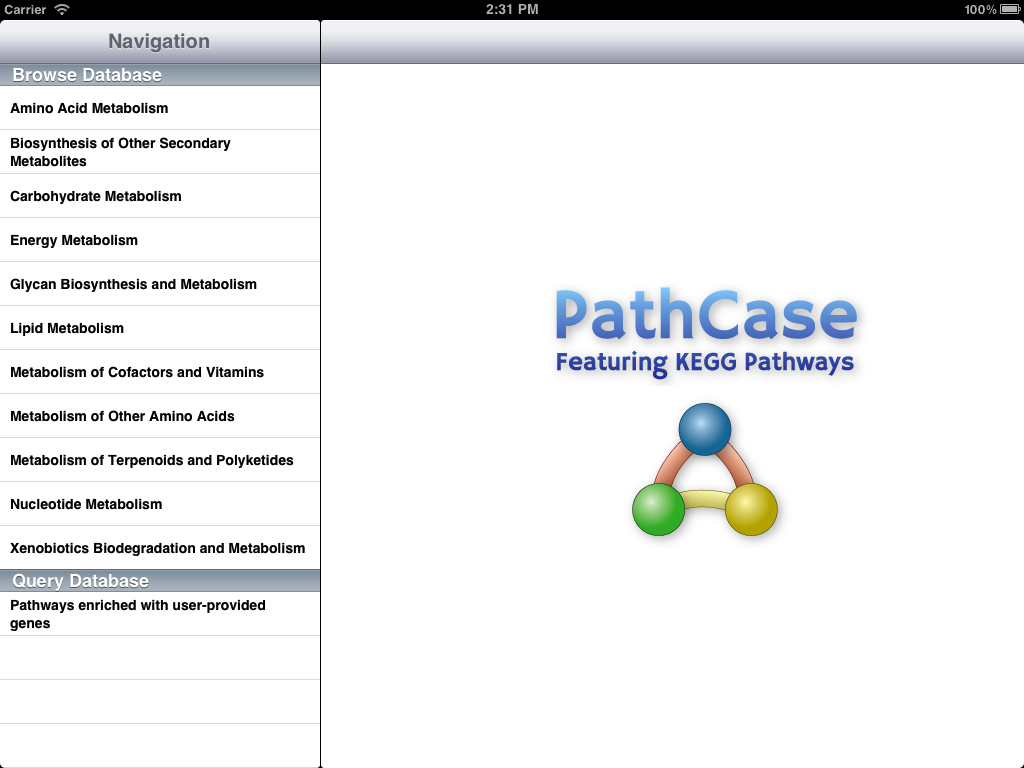
\includegraphics[width=\textwidth]{kegg/figures/screenshot_list}}
    \caption{\label{fig:kegg_screenshot_list} List of pathway categories on
    the main screen of \keggapp}
\end{figure}

\begin{figure}
    \center{
        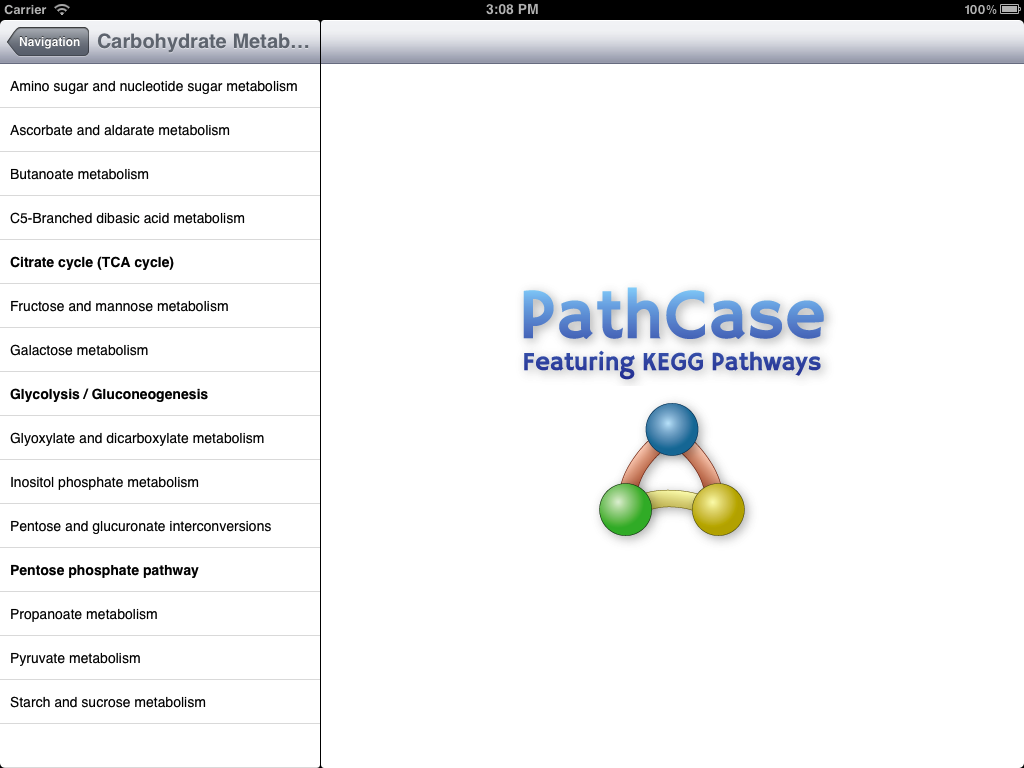
\includegraphics[width=\textwidth]{kegg/figures/screenshot_sublist}}
    \caption{\label{fig:kegg_screenshot_sublist} List of pathways in the
    ``Carbohydrate Metabolism'' category of \keggapp}
\end{figure}

\keggapp divides the screen into a master-detail interface (see
\ref{sect:ipad_container_views}. The sidebar (master view) provides navigation
functionality and metadata for the currently selected object. The detail view
displays content chosen from the sidebar, such as documentation or a graph view.
When the device is in the landscape orientation, the master view is shown to the
left of the detail view.  In portrait orientation, it is accessed via a button
in the upper left corner of the screen. This interface is described visually in
figure \ref{fig:master_detail}.

The home screen of \keggapp displays a list of pathway categories in the
sidebar. Selecting a category takes the user to a list of pathways. These lists
are shown in figures \ref{fig:kegg_screenshot_pathway} and
\ref{fig:kegg_screenshot_sublist}.  (Unlike \mawapp, \keggapp can
display pathways that do not have frozen layouts.)

Selecting a pathway from the list opens the graph view of that pathway in the
detail view. This graph view can be panned and zoomed by touch. The view for
the TCA cycle is shown in figure \ref{fig:kegg_screenshot_pathway}. A labeled
diagram of the same view is shown in figure \ref{fig:kegg_pathway_diagram}.

\begin{figure}[hbt]
    \center{
        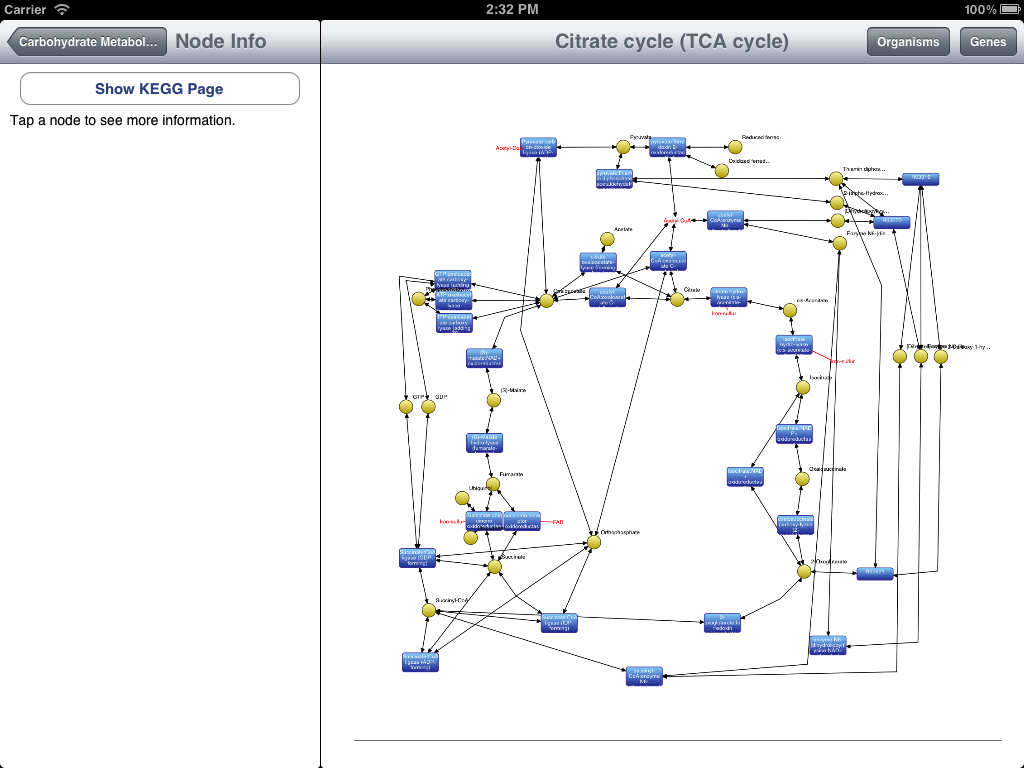
\includegraphics[width=\textwidth]{kegg/figures/screenshot_pathway}}
    \caption{\label{fig:kegg_screenshot_pathway} Scrolling, zooming view of
    the TCA cycle}
\end{figure}

\begin{figure}[hbt]
    \center{
        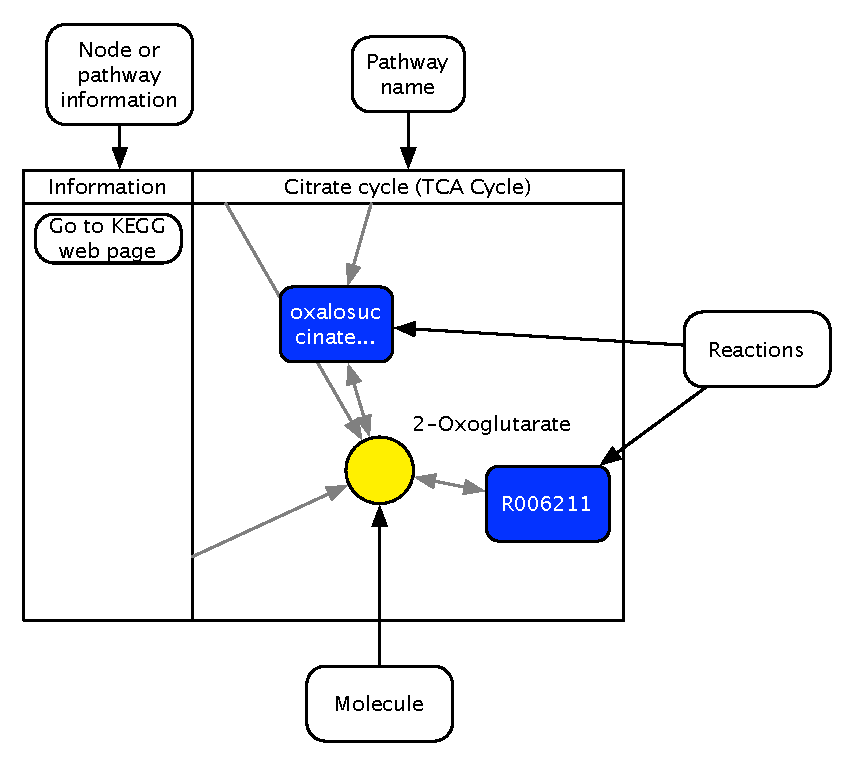
\includegraphics[width=4in]{kegg/figures/pathway_diagram}}
    \caption{\label{fig:kegg_pathway_diagram} Parts of the KEGG pathway browsing
    interface}
\end{figure}

\begin{figure}[hbt]
    \center{
        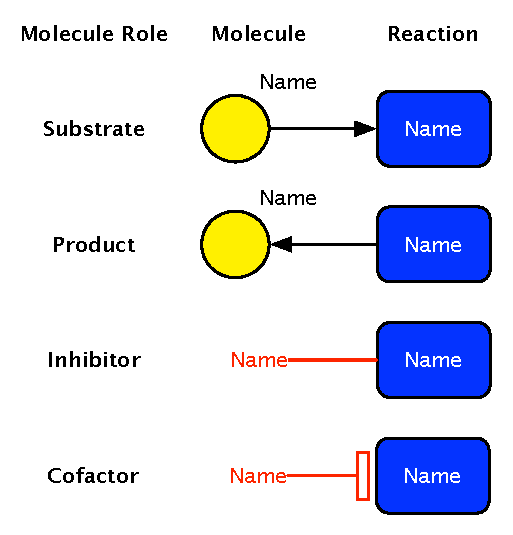
\includegraphics[width=3in]{kegg/figures/node_legend}}
    \caption{\label{fig:kegg_node_legend} Meanings of KEGG pathway node shapes}
\end{figure}

As in \mawapp, rectangular nodes represent reactions and the rest of the nodes
represent molecules. A key for the different node types is shown in figure
\ref{fig:kegg_node_legend}.

The graph view differs from \mawappp graph view in several ways. The first
is the presence of the sidebar, which displays information about the user's
current selection. If no node is selected, it displays a button to show the KEGG
database web page for the pathway. (One example page is shown in figure
\ref{fig:kegg_screenshot_kegg_web_site}.)

\begin{figure}[hbt]
    \center{
        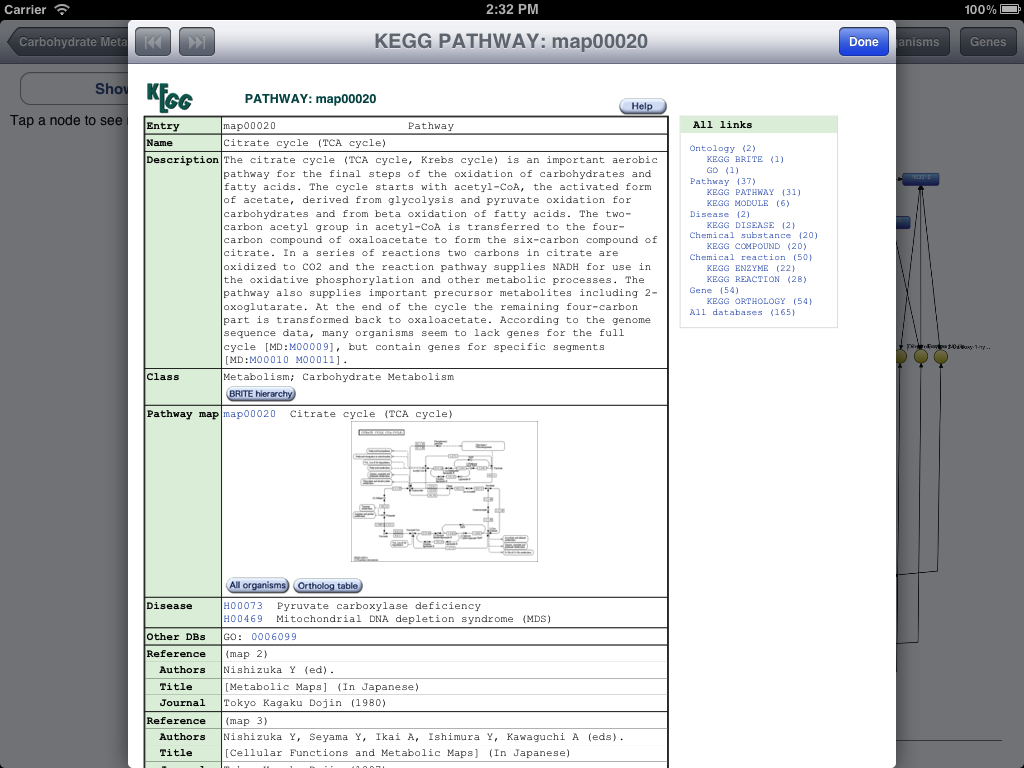
\includegraphics[width=\textwidth]{kegg/figures/screenshot_kegg_web_site}}
    \caption{\label{fig:kegg_screenshot_kegg_web_site} KEGG web page for the TCA
    cycle, displayed by tapping the sidebar button}
\end{figure}

If the user taps a node, the node is ``selected,'' and the sidebar shows a
longer description of the node.  This differs from \mawappp behavior of using
a popover to display the longer description. When a node is selected, any other
node that is not connected to it by one hop is made transparent to make the
node's connections easier to see.  Figure
\ref{fig:kegg_screenshot_selection_no_info} shows an example of this behavior.

\begin{figure}[hbt]
    \center{
        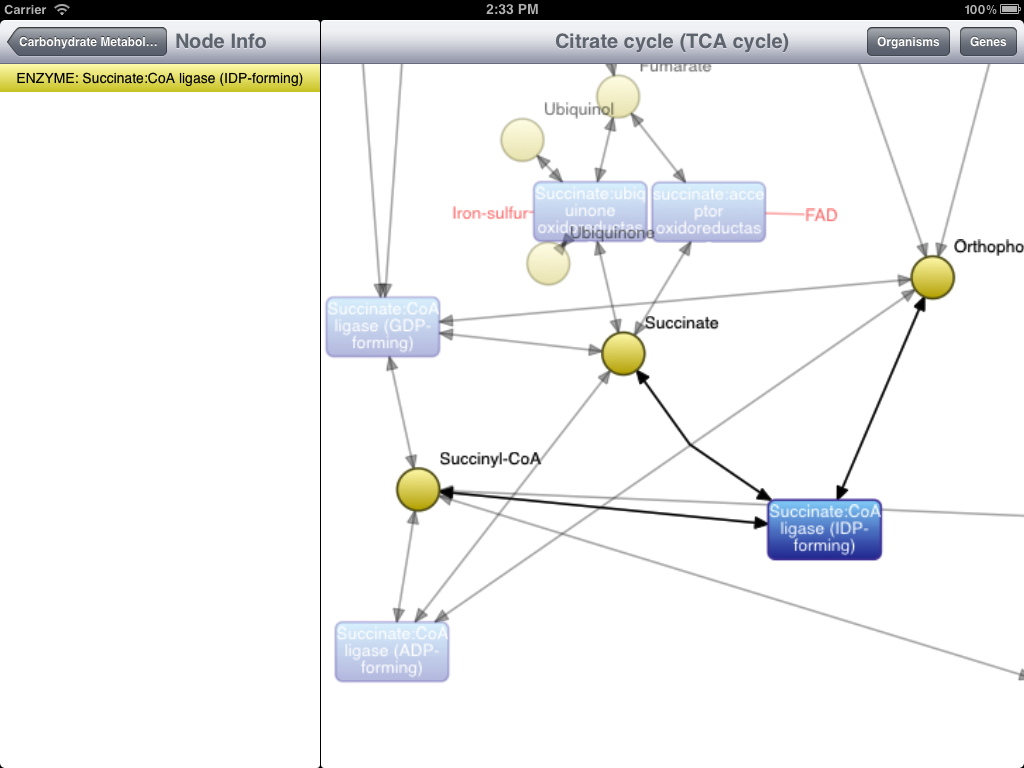
\includegraphics[width=\textwidth]{kegg/figures/screenshot_selection_no_info}}
    \caption{\label{fig:kegg_screenshot_selection_no_info} Sidebar showing
    long description of a node in \keggapp}
\end{figure}

The second major difference is the addition of the ``Organisms'' button in the
upper right corner. This button triggers a popover which allows the user to
activate and deactivate organisms. If a reaction is not present in any activated
organism, it is made partially transparent.

The organism hierarchy menu is shown in figure
\ref{fig:kegg_screenshot_animals_only_list}. The graph view corresponding to the
selection is shown in figure \ref{fig:kegg_screenshot_animals_only_graph}.

\begin{figure}[hbt]
    \center{
        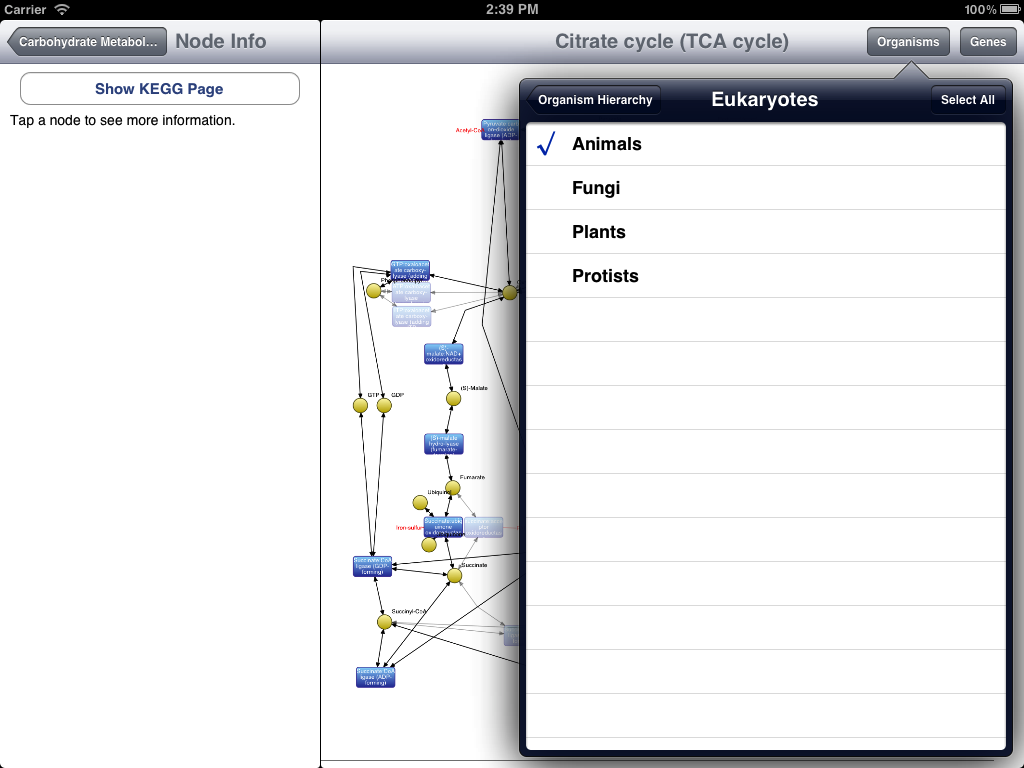
\includegraphics[width=\textwidth]{kegg/figures/screenshot_animals_only_list}}
    \caption{\label{fig:kegg_screenshot_animals_only_list} Organism hierarchy
    menu with only Eukaryotes $\rightarrow$ Animals activated}
\end{figure}

\begin{figure}[hbt]
    \center{
        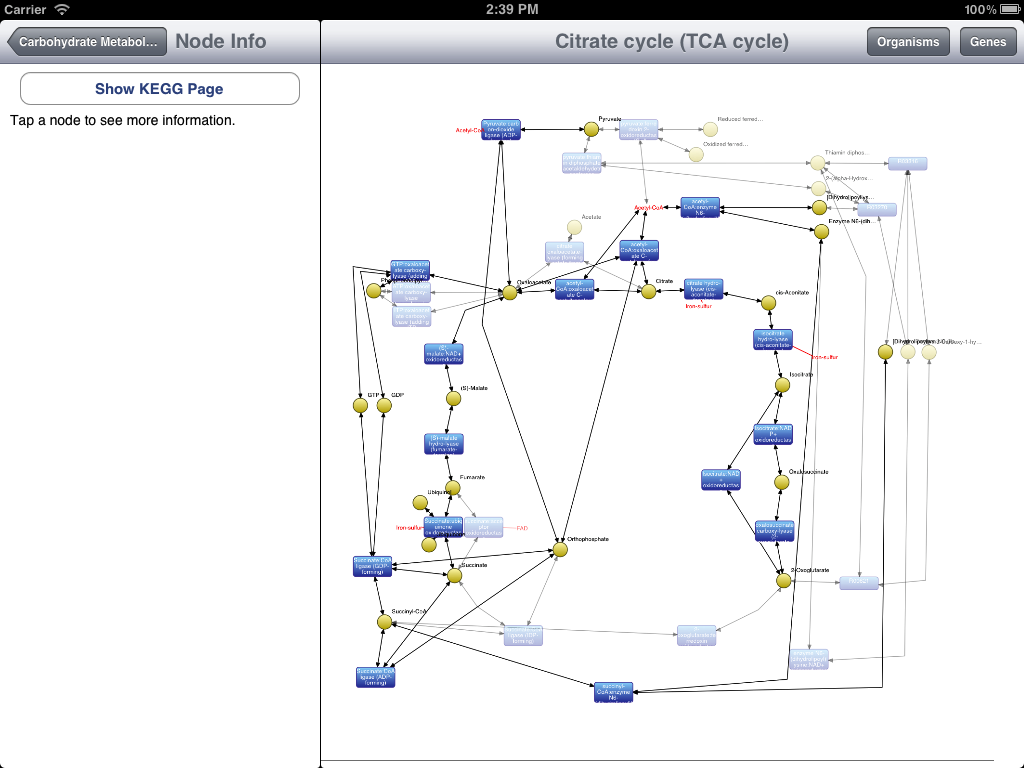
\includegraphics[width=\textwidth]{kegg/figures/screenshot_animals_only_graph}}
    \caption{\label{fig:kegg_screenshot_animals_only_graph} Graph view with only
    reactions for Eukaryotes $\rightarrow$ Animals activated}
\end{figure}

\subsection{ENZYME Database Information}

In addition to displaying a node's long description from PathCase KEGG, \keggapp
uses data from the ENZYME enzyme nomenclature database to show more information
for reactions for which EC numbers are available.

ENZYME's data comes from the recommendations of the Nomenclature Committee of
the International Union of Biochemistry and Molecular Biology (IUBMB)
\cite{enzyme-database}. An example of ENZYME information in the sidebar is shown
in figure \ref{fig:kegg_screenshot_selection_info}, including alternate names,
catalytic activity, cofactors, and more.

\begin{figure}[hbt]
    \center{
        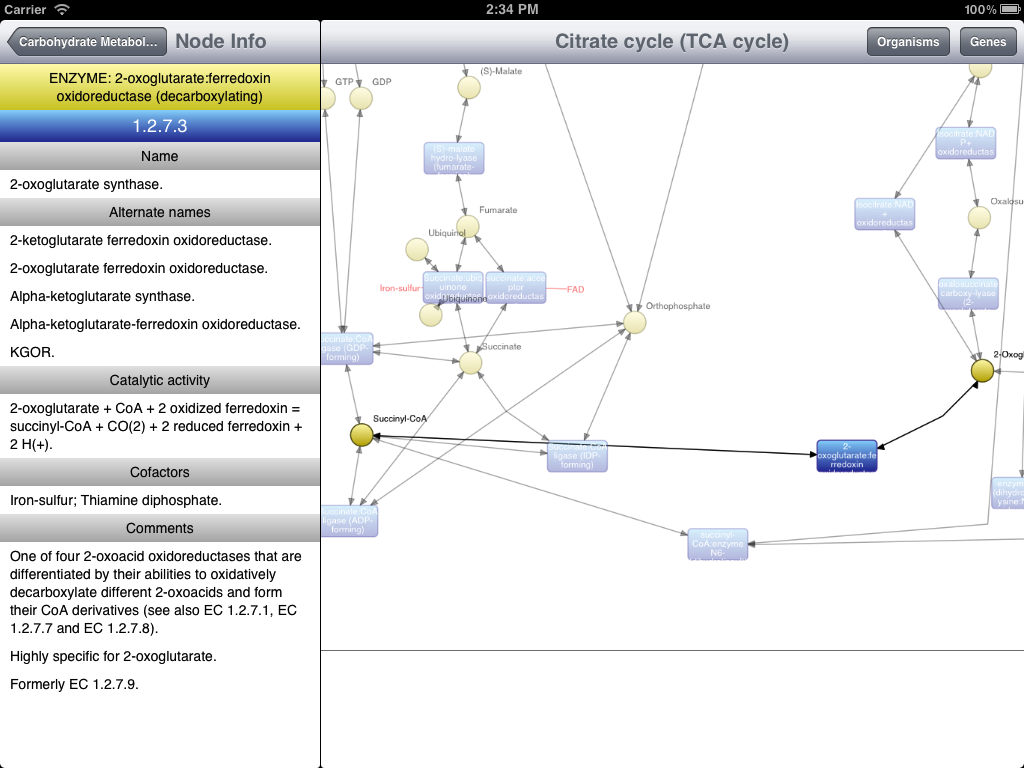
\includegraphics[width=\textwidth]{kegg/figures/screenshot_selection_info}}
    \caption{\label{fig:kegg_screenshot_selection_info} Sidebar showing
    information from the ENZYME database for the reaction ``2-oxoglutarate
    synthase''}
\end{figure}
